\documentclass[tikz,border=6pt]{standalone}
\usepackage{tikz}
\usetikzlibrary{arrows.meta,positioning,calc}
\definecolor{ink}{HTML}{263238}
\definecolor{blue}{HTML}{2F6BBD}
\definecolor{bluefill}{HTML}{EAF2FF}
\definecolor{green}{HTML}{4C8A62}
\definecolor{greenfill}{HTML}{EAF6ED}
\definecolor{orange}{HTML}{C98232}
\definecolor{orangefill}{HTML}{FFF3E5}
\definecolor{purple}{HTML}{71549A}
\definecolor{purplefill}{HTML}{F3EDFF}
\definecolor{gray}{HTML}{65727B}
\definecolor{grayfill}{HTML}{F3F5F6}
\tikzset{
  cardbase/.style={rounded corners=2pt, line width=0.7pt, minimum width=3.15cm, minimum height=1.04cm, align=left, inner xsep=7pt, inner ysep=5pt, font=\sffamily\footnotesize, text=ink},
  cardgray/.style={cardbase, draw=gray, fill=grayfill},
  cardgreen/.style={cardbase, draw=green, fill=greenfill},
  cardblue/.style={cardbase, draw=blue, fill=bluefill},
  cardorange/.style={cardbase, draw=orange, fill=orangefill},
  cardpurple/.style={cardbase, draw=purple, fill=purplefill},
  flow/.style={-{Latex[length=2mm]}, line width=0.8pt, draw=#1},
  note/.style={font=\sffamily\scriptsize, text=gray, align=center}
}
\begin{document}
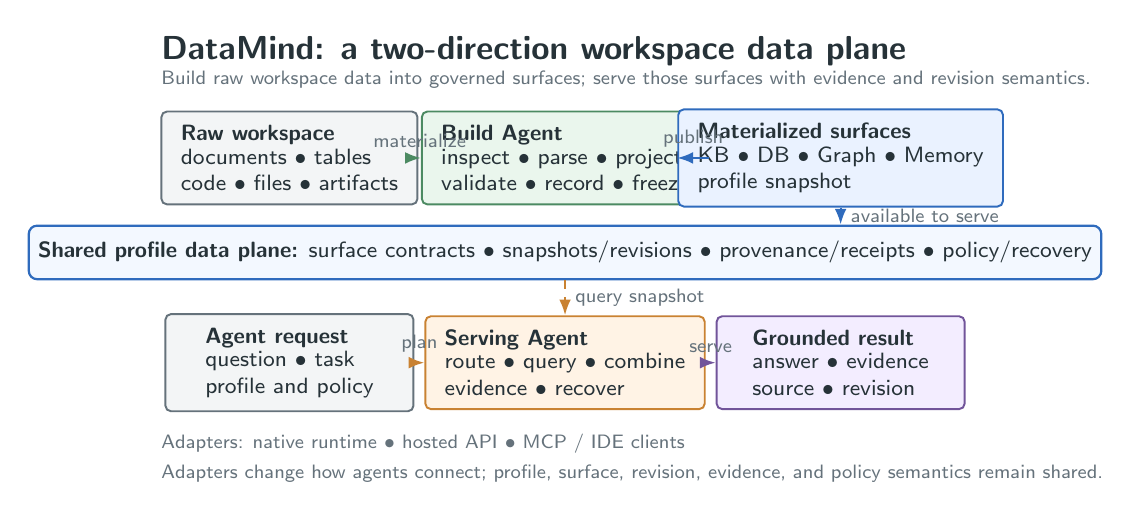
\begin{tikzpicture}[x=1cm,y=1cm]
\node[anchor=west, font=\sffamily\bfseries\large, text=ink] at (0,5.6) {DataMind: a two-direction workspace data plane};
\node[anchor=west, note, align=left] at (0,5.24) {Build raw workspace data into governed surfaces; serve those surfaces with evidence and revision semantics.};

% Build direction
\node[cardgray] (raw) at (1.75,4.25) {\textbf{Raw workspace}\\[-1pt]documents $\bullet$ tables\\code $\bullet$ files $\bullet$ artifacts};
\node[cardgreen] (build) at (5.25,4.25) {\textbf{Build Agent}\\[-1pt]inspect $\bullet$ parse $\bullet$ project\\validate $\bullet$ record $\bullet$ freeze};
\node[cardblue] (surfaces) at (8.75,4.25) {\textbf{Materialized surfaces}\\[-1pt]KB $\bullet$ DB $\bullet$ Graph $\bullet$ Memory\\profile snapshot};
\draw[flow=green] (raw.east) -- node[above,note]{materialize} (build.west);
\draw[flow=blue] (build.east) -- node[above,note]{publish} (surfaces.west);

% Shared plane
\node[draw=blue, fill=bluefill!55, rounded corners=3pt, line width=0.8pt, minimum width=10.15cm, minimum height=0.68cm, align=center, font=\sffamily\footnotesize, text=ink] (plane) at (5.25,3.05) {\textbf{Shared profile data plane:} surface contracts $\bullet$ snapshots/revisions $\bullet$ provenance/receipts $\bullet$ policy/recovery};
\draw[flow=blue, dashed] (surfaces.south) -- node[right,note]{available to serve} (plane.north -| surfaces.south);

% Serve direction
\node[cardgray] (request) at (1.75,1.65) {\textbf{Agent request}\\[-1pt]question $\bullet$ task\\profile and policy};
\node[cardorange] (serve) at (5.25,1.65) {\textbf{Serving Agent}\\[-1pt]route $\bullet$ query $\bullet$ combine\\evidence $\bullet$ recover};
\node[cardpurple] (answer) at (8.75,1.65) {\textbf{Grounded result}\\[-1pt]answer $\bullet$ evidence\\source $\bullet$ revision};
\draw[flow=orange] (request.east) -- node[above,note]{plan} (serve.west);
\draw[flow=purple] (serve.east) -- node[above,note]{serve} (answer.west);
\draw[flow=orange, dashed] (plane.south -| serve.north) -- node[right,note]{query snapshot} (serve.north);

\node[anchor=west, font=\sffamily\scriptsize, text=gray] at (0,0.62) {Adapters: native runtime $\bullet$ hosted API $\bullet$ MCP / IDE clients};
\node[anchor=west, font=\sffamily\scriptsize, text=gray] at (0,0.24) {Adapters change how agents connect; profile, surface, revision, evidence, and policy semantics remain shared.};
\end{tikzpicture}
\end{document}
